\documentclass{article}
\usepackage[pdftex]{graphicx}
\usepackage{subcaption}
\usepackage{fullpage}

\begin{document}

\title{cta200 Project}
\author{Sabrina Madsen}
\date{May 18, 2018}
\maketitle


\section{Introduction}

In this project the caustic curves, critical curves, and image position will be determined and plotted for light from a source star lensed by a single-planet solar system.

When light from a background (source) star passes near massive foreground objects (lens objects) the light will be lensed by the foreground star or planet. This will distort the image of the source star, creating multiple images of the source at various positions around the lens objects. These images will be magnified and distorted. In order to determine how these images are distorted one must first look at the lens equation, given by Eq.~(\ref{eq:Lens}), for the case of two lens objects.

\begin{equation}
\zeta = z + \frac{\epsilon_1}{\bar{z}_{m,1}-\bar{z}}+ \frac{\epsilon_2}{\bar{z}_{m,2}-\bar{z}}
\label{eq:Lens}
\end{equation}

\noindent where $\zeta$ is the source position, $z$ is the image position, $z_{m,1}$ and $z_{m,2}$ are the position of the first and second lensing objects, star and planet, respectively. These values are complex, the real portion gives the $x$ coordinate and the imaginary portion gives the $y$ coordinate. Furthermore, in this notation a `bar' above a variable denotes its complex conjugate. $\epsilon_1$ and $\epsilon_2$ are the ratios of the mass of the first lensing object ($m_1$) and the mass of the second lensing object ($m_2$), respectively, to the total mass of the lens system, as given by Eqs.~(\ref{eq:e1}) and (\ref{eq:e2}) respectively.

\begin{minipage}[c]{0.45\textwidth}
\begin{equation}
\epsilon_1=\frac{m_1}{m_1+m_2}
\label{eq:e1}
\end{equation}
\end{minipage}
\begin{minipage}[c]{0.5\textwidth}
\begin{equation}
\epsilon_2= \frac{m_2}{m_1+m_2}
\label{eq:e2}
\end{equation}
\end{minipage}

\smallskip

Lensing can create and magnify multiple images of the source, the magnification of each image, $A_j$, is given by the inverse of the determinant of the Jacobian, $J$, of the lens equation at the position of that image, $z_j$, as seen in Eqs.~(\ref{eq:A_j}) and~(\ref{eq:detJ}).

\begin{minipage}{0.45\textwidth}
\begin{equation}
A_j = \frac{1}{detJ}\Big|_{z = z_j}
\label{eq:A_j}
\end{equation}
\end{minipage}
\begin{minipage}{0.5\textwidth}
\begin{equation}
detJ = 1-\frac{\partial \zeta}{\partial \bar{z}} \overline{\frac{\partial \zeta}{\partial\bar{z}}}
\label{eq:detJ}
\end{equation}
\end{minipage}

\section{Caustic and Critical Curves}
\smallskip

\begin{equation}
\frac{\epsilon_1}{(z-z_{m,1})^2}+\frac{\epsilon_2}{(z-z_{m,2})^2}=e^{i \phi}
\label{eq:Critical}
\end{equation}

\smallskip

The caustic curves for a particular lensing system are closed curves which denote the positions at which the Jacobian of the lens equation equals zero. Furthermore, the critical curves are the images of the caustic curves. The positions of the critical curves can be determined by solving the parametric equation, Eq.~(\ref{eq:Critical}), for the critical curve positions, $z$, for each value of $\phi$ between 0 and 2$\pi$. This resulted in a fourth order polynomial in $z$, which was solved in python, with the NumPy module, by using the numpy.roots() command, as seen in the python code provided. $z$ was found to have three or four roots, for each value of $\phi$, which were saved to a list and plotted as the critical curves. These results were then substituted into the lens equation in order to find the positions of the caustic curves. Note that during this analysis, the star, $m_1$, was assumed to be at the origin (i.e. $z_{m,1}$ = 0) and the planet, $m_2$, was set to be on the x-axis (that is, $z_{m,2}=x$). Furthermore, the mass ratio between the planet and star, $m_1/m_2$, was set to be 0.003. The resulting caustic and critical curves can be seen in Fig.~\ref{fig:Caustic_Curves} for various distances, $x$ between the lens star and planet.


\begin{figure}[h]
\centering
\begin{subfigure}{.5\textwidth}
  \begin{minipage}{0.1\textwidth}
    \caption{} \label{fig:Caustic_x=0_25}
  \end{minipage}\hfill
\begin{minipage}[c]{0.85\textwidth}
    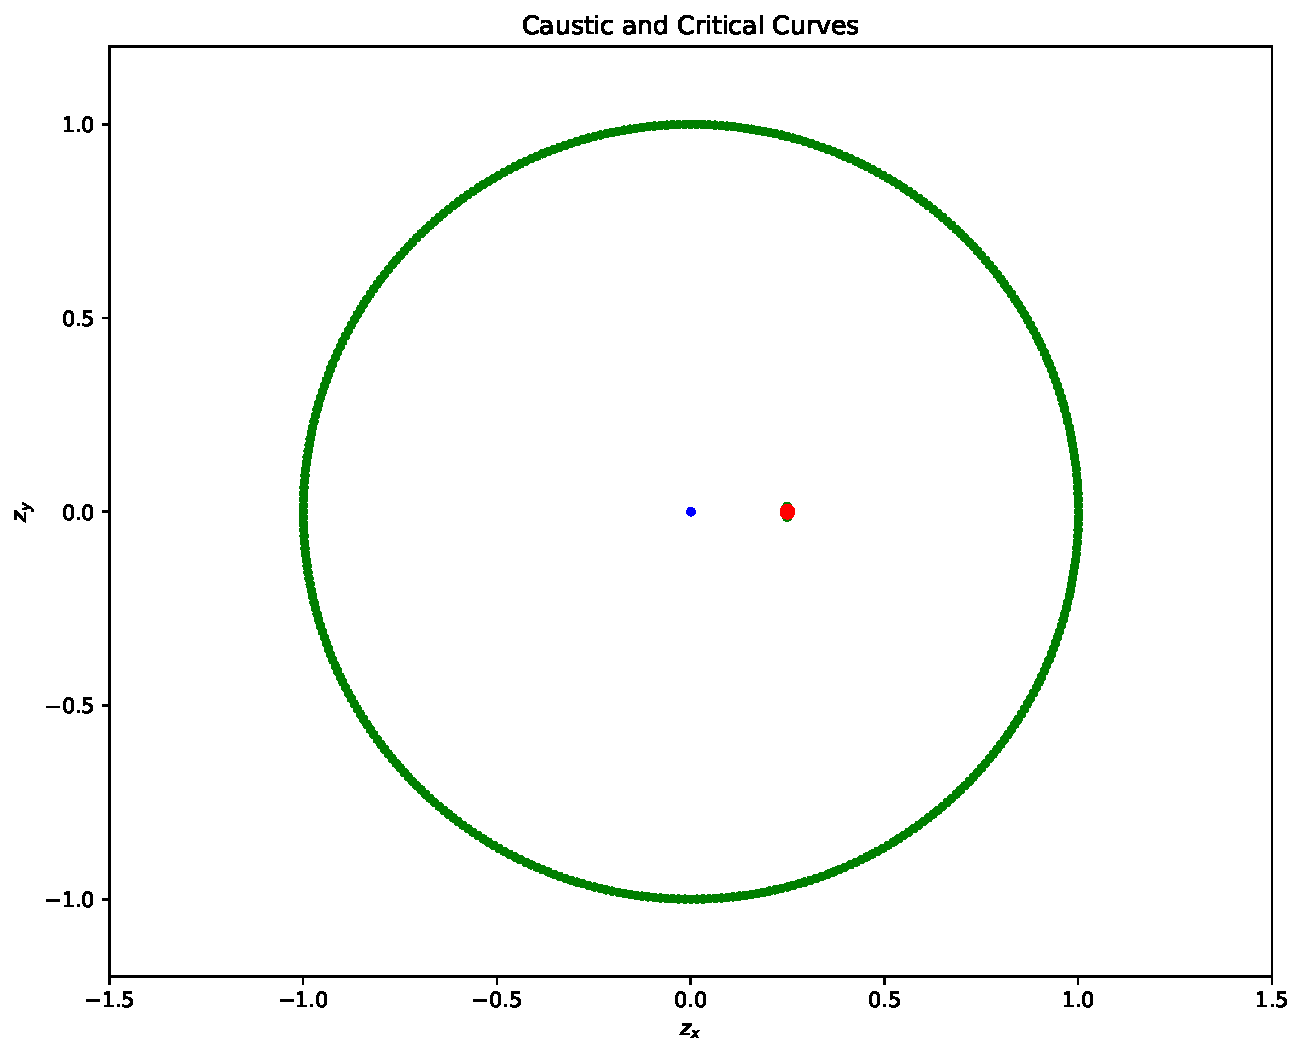
\includegraphics[width=7 cm]{Critical_and_Caustic_Curves_x_0_25.pdf}
  \end{minipage}\hfill
\end{subfigure}%
\begin{subfigure}{.5\textwidth}
  \begin{minipage}{0.1\textwidth}
    \caption{} \label{fig:Caustic_x=0_9}
  \end{minipage}\hfill
\begin{minipage}[c]{0.85\textwidth}
    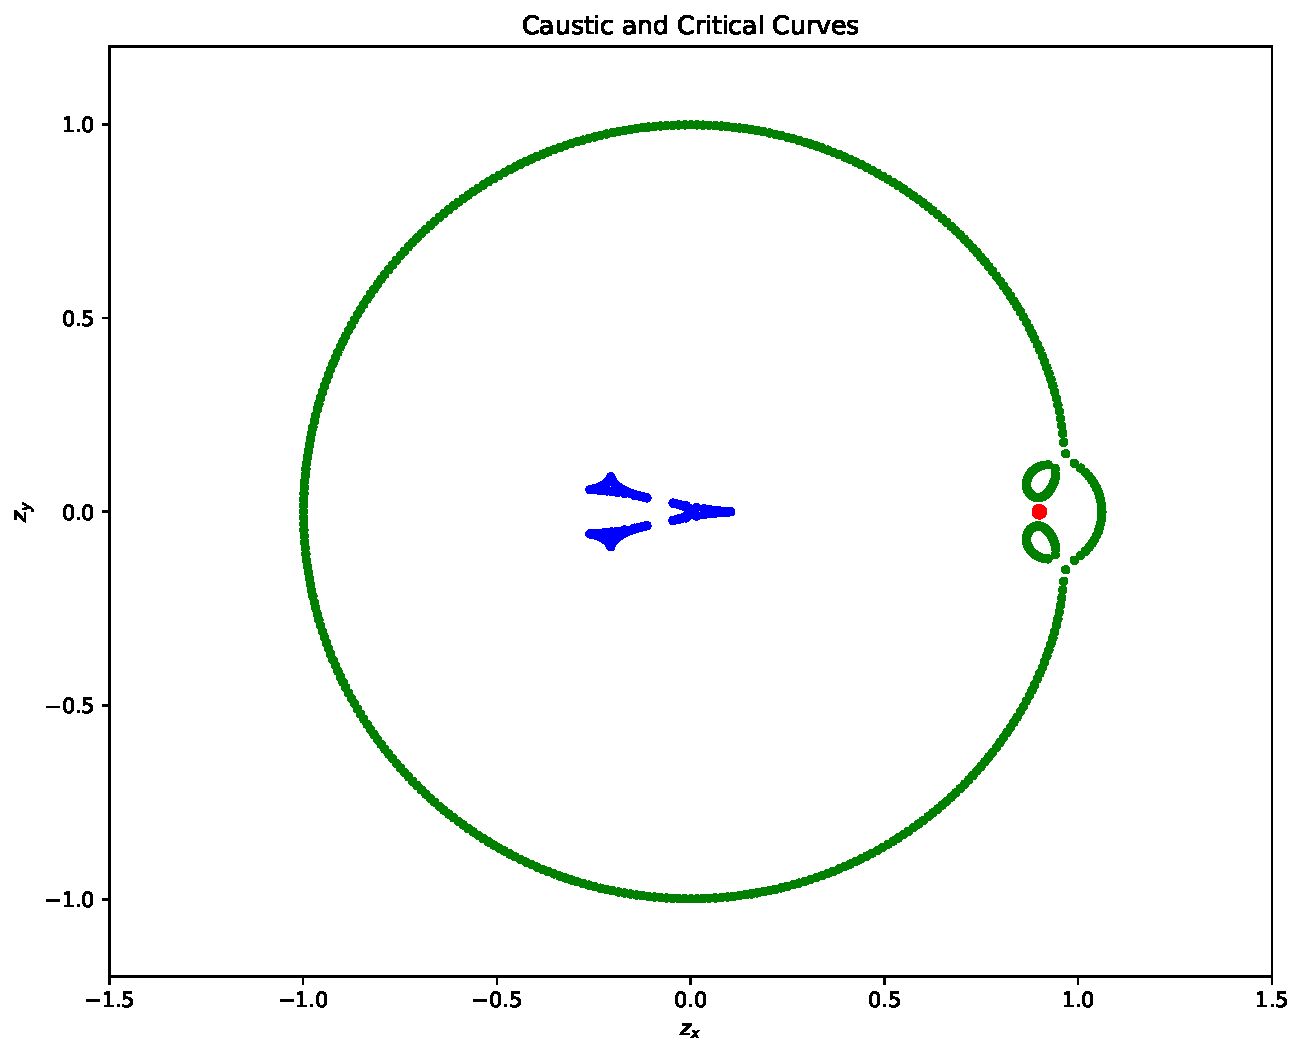
\includegraphics[width=7 cm]{Critical_and_Caustic_Curves_x_0_9.pdf}
  \end{minipage}\hfill
\end{subfigure} \\
\begin{subfigure}{.5\textwidth}
  \begin{minipage}{0.1\textwidth}
    \caption{} \label{fig:Caustic_x=1}
  \end{minipage}\hfill
\begin{minipage}[c]{0.85\textwidth}
    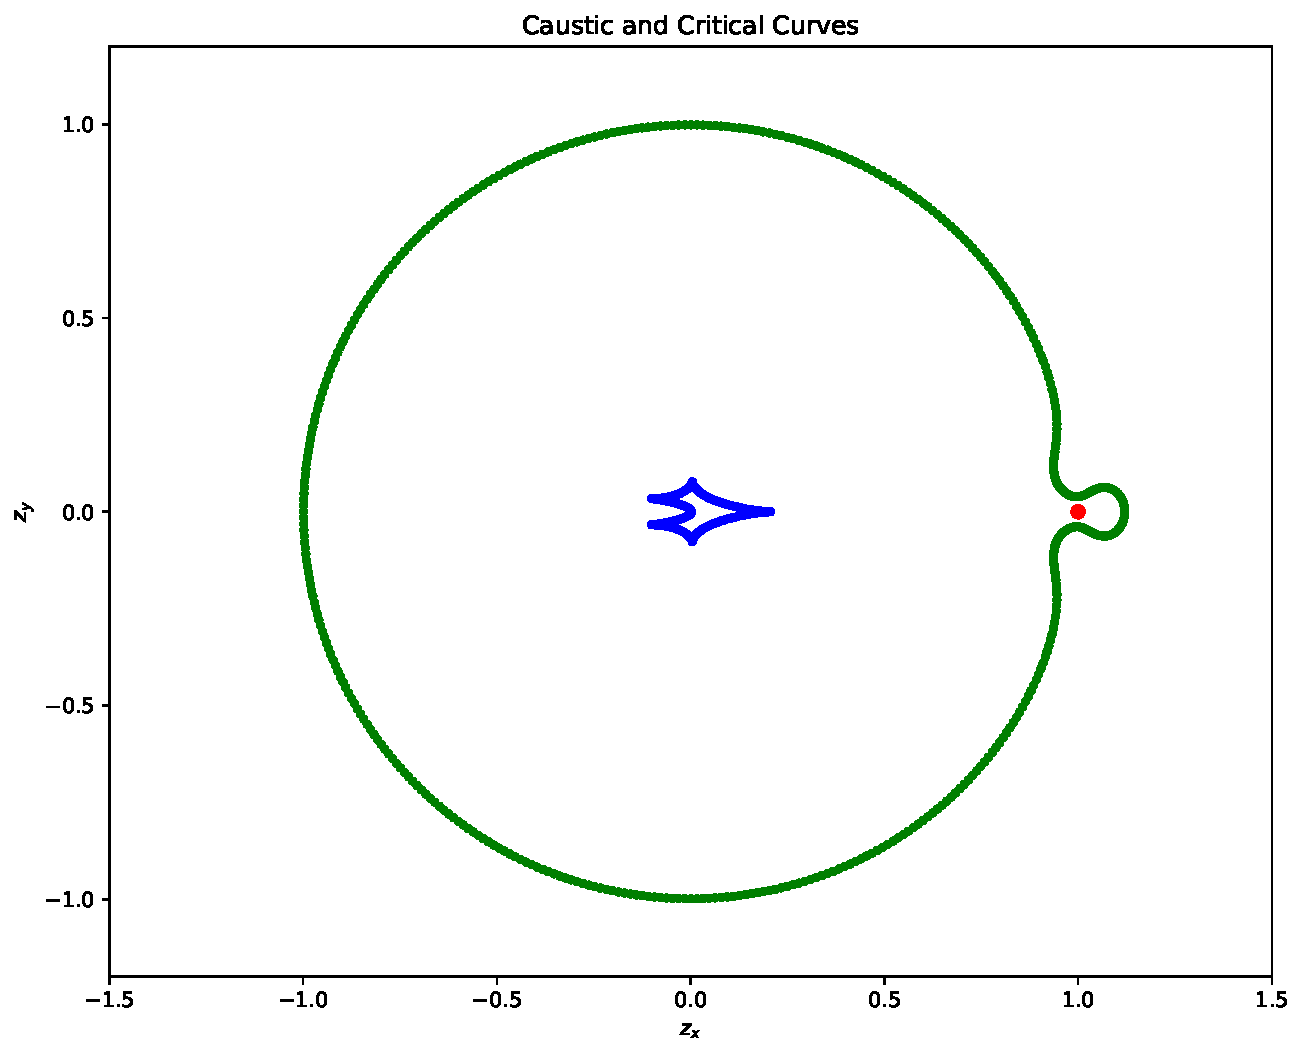
\includegraphics[width=7 cm]{Critical_and_Caustic_Curves_x_1.pdf}
  \end{minipage}\hfill
\end{subfigure}%
\begin{subfigure}{.5\textwidth}
  \begin{minipage}{0.1\textwidth}
    \caption{} \label{fig:Caustic_x=1_3}
  \end{minipage}\hfill
\begin{minipage}[c]{0.85\textwidth}
    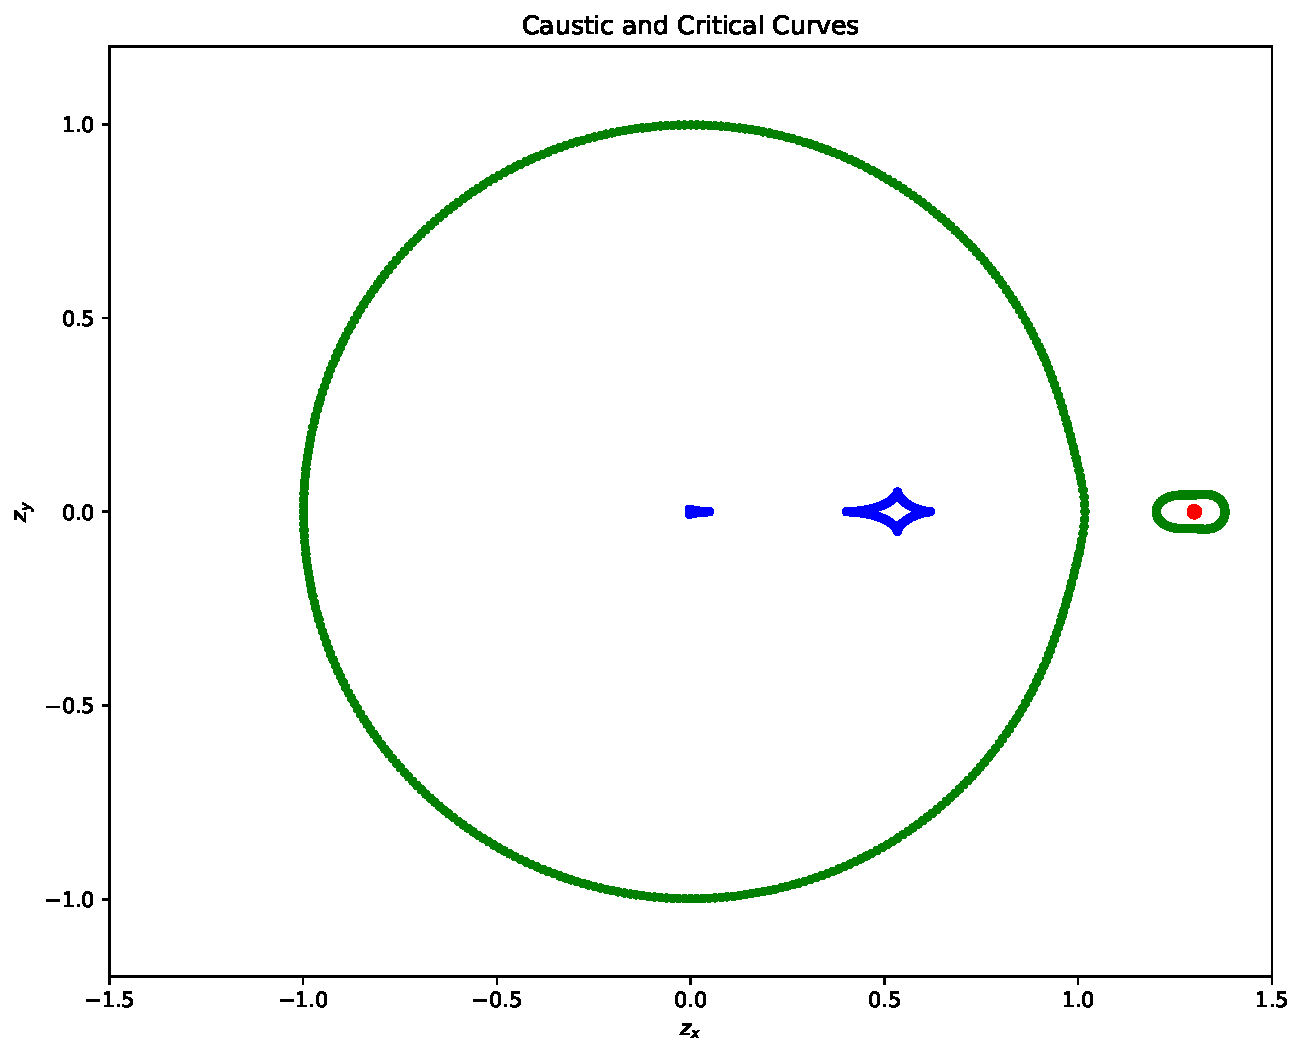
\includegraphics[width=7 cm]{Critical_and_Caustic_Curves_x_1_3.pdf}
  \end{minipage}\hfill
\end{subfigure}%
\captionsetup{justification=centering}
\caption{\label{fig:Caustic_Curves} Caustic curves, plotted in blue, and critical curves, plotted in green, are shown for various distances between the star, positioned at the origin, and the planet, denoted by the red circle. Figures~\ref{fig:Caustic_x=0_25}, \ref{fig:Caustic_x=0_9}, \ref{fig:Caustic_x=1}, and \ref{fig:Caustic_x=1_3} show the critical and caustic curves for distances of 0.25~$\theta_E$, 0.9~$\theta_E$, 1~$\theta_E$, and 1.3~$\theta_E$, respectively, between the star and planet. Here $\theta_E$ denotes the Einstein radius of the lens star.}
\end{figure}


\section{Image Positions and Magnification}

When a source star passes behind the lens, its image will be distorted, creating multiple images which are magnified compared to the source. 

In order to determine the position of these images, $z$, for a particular source position, $\zeta$, the lens equation, given by Eq.~(\ref{eq:Lens}) was used. The lens equation however, has two unknown variables: $z$ and $\bar{z}$. In order to eliminate one of these variables the complex conjugate of the lens equation was taken and was solved for $\bar{z}$, as seen in Eq.~(\ref{eq:LensBar}).


\begin{equation}
\bar{\zeta}=\bar{z} - \frac{\epsilon_1}{z-z_{m,1}} - \frac{\epsilon}{z-z_{m,2}} \leftrightarrow \bar{z} =\frac{\bar{\zeta}(z-z_{m,1})(z-z_{m,2})+\epsilon_1(z-z_{m,2}) + \epsilon_2(z-z_{m,1})}{(z-z_{m,1})(z-z_{m,2})}
\label{eq:LensBar}
\end{equation}

\noindent This value of $\bar{z}$ was then substituted back into the lens equation resulting in a fifth order polynomial in $z$. During this analysis the position of the lens star, $z_{m,1}$ was again set to 0, the position of the source $\zeta$ was chosen to move along a horizontal line (i.e. its $x$ position was allowed to vary while its $y$ position was held constant at 0.2~$\theta_E$). The position of the planet however, was not set to be on the x-axis since the displacement from the lens star to planet is not necessarily parallel to the trajectory of the source star. 

The fifth order polynomial was then solved for the image position, $z$. This resulted in five solutions however, some of the solutions were not physical, that is, five images were not actually produced. In order to determine which solutions were physical, the $z$ values were entered into the lens equation. If the $z$ values satisfied the lens equation they were plotted as the image positions as seen in Fig~\ref{fig:Image_and_Magnification}. This process was repeated for the entire trajectory of the source moving past the lens star as seen in the python code provided.

The total magnification of the source object is defined as the sum of the magnification of each of the images, given by Eq~($\ref{eq:A_j}$). In order to determine the magnification, the determinant of the Jacobian of the lens equation first had to be determined using Eq.~(\ref{eq:detJ}). The result was then used in Eq~(\ref{eq:A_j}) for each image to obtain $A_j$. The sum of $A_j$ was taken and plotted as a function of the x-position of the source star as it transited behind the lens objects as seen in Fig~\ref{fig:Image_and_Magnification}. The magnification, shown in blue, is perturbed from the single lens magnification, shown by the red dotted line. Therefore by measuring the magnitude and positions of the images of a background star lensed by a foreground solar system, planets in the lens system can be detected.

\begin{figure}[h]
\centering
\begin{subfigure}{.5\textwidth}
  \begin{minipage}{0.1\textwidth}
    \caption{} \label{fig:Image_1_2_0_5j}
  \end{minipage}\hfill
\begin{minipage}[c]{0.85\textwidth}
    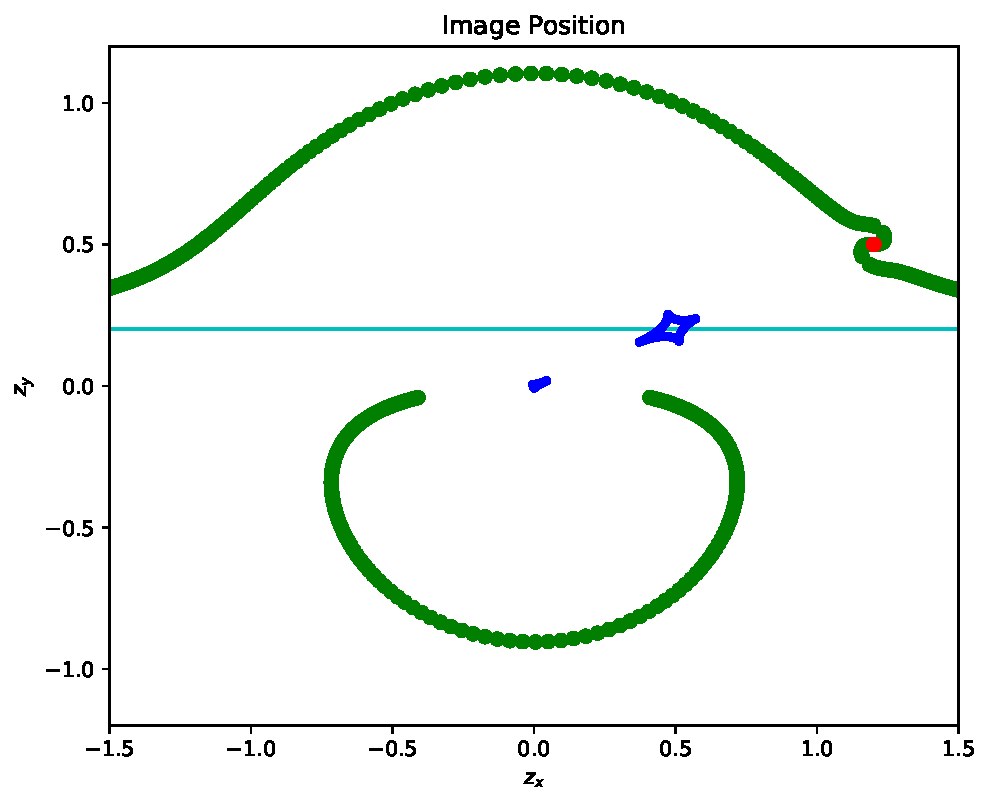
\includegraphics[width=7 cm]{Image_and_Caustic_Curves_x_1_2_0_5j.pdf}
  \end{minipage}\hfill
\end{subfigure}%
\begin{subfigure}{.5\textwidth}
  \begin{minipage}{0.1\textwidth}
    \caption{} \label{fig:Magnification_1_2_0_5j}
  \end{minipage}\hfill
\begin{minipage}[c]{0.85\textwidth}
    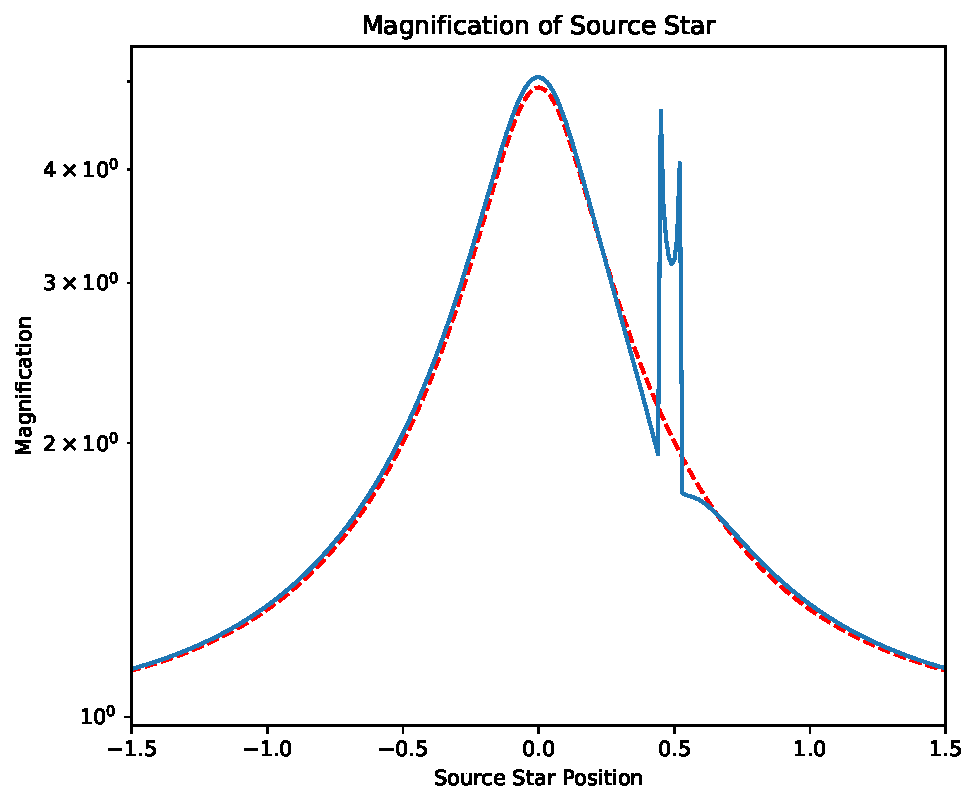
\includegraphics[width=7 cm]{Magnification_x_1_2_0_5j.pdf}
  \end{minipage}\hfill
\end{subfigure} \\
\begin{subfigure}{.5\textwidth}
  \begin{minipage}{0.1\textwidth}
    \caption{} \label{fig:Image_1_2_n0_5j}
  \end{minipage}\hfill
\begin{minipage}[c]{0.85\textwidth}
    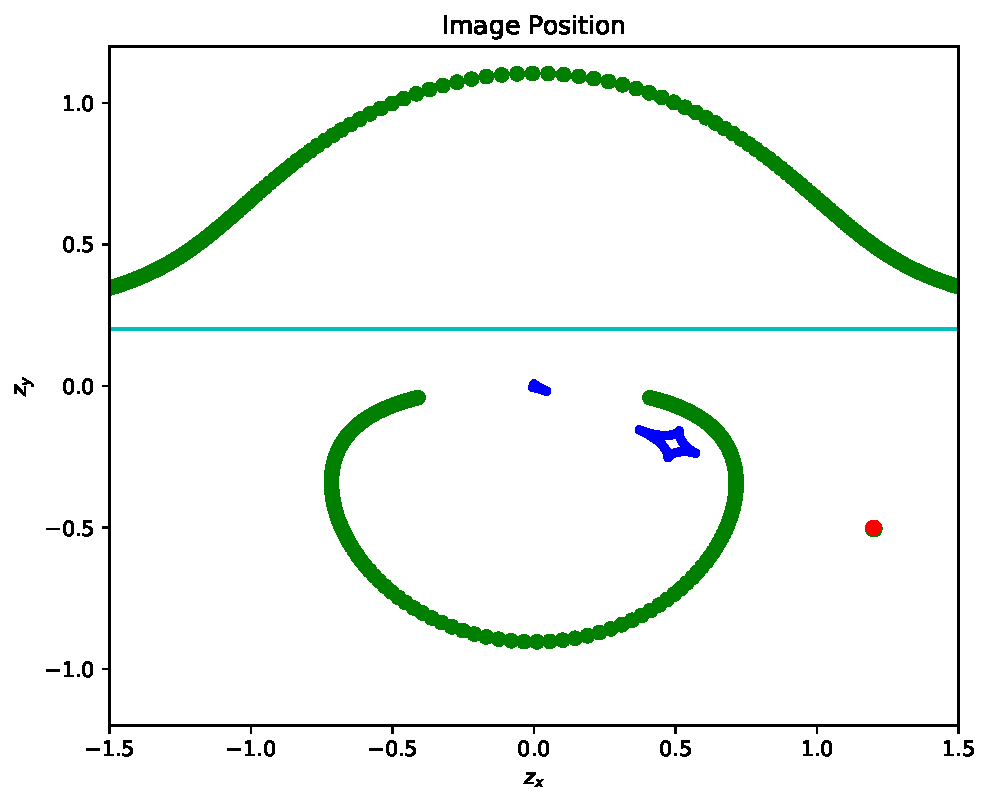
\includegraphics[width=7 cm]{Image_and_Caustic_Curves_x_1_2_-0_5j.pdf}
  \end{minipage}\hfill
\end{subfigure}%
\begin{subfigure}{.5\textwidth}
  \begin{minipage}{0.1\textwidth}
    \caption{} \label{fig:Magnification_1_2_-0_5j}
  \end{minipage}\hfill
\begin{minipage}[c]{0.85\textwidth}
    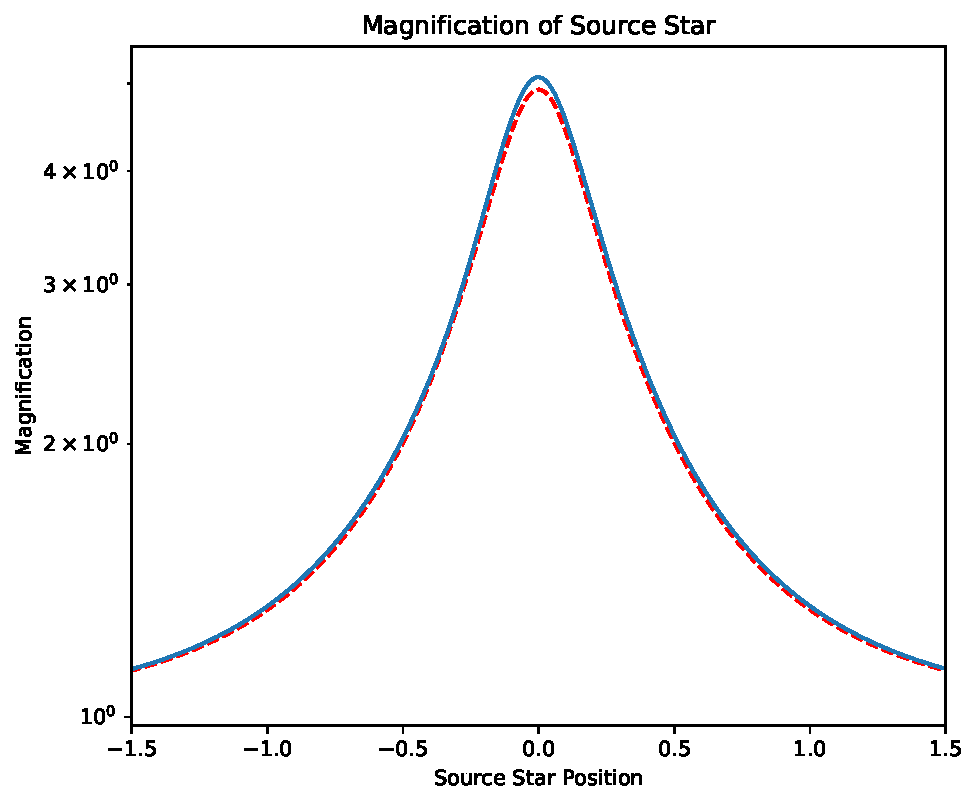
\includegraphics[width=7 cm]{Magnification_x_1_2_-0_5j.pdf}
  \end{minipage}\hfill
\end{subfigure} \\
\begin{subfigure}{.5\textwidth}
  \begin{minipage}{0.1\textwidth}
    \caption{} \label{fig:Image_sqrt3_2_n0_5j}
  \end{minipage}\hfill
\begin{minipage}[c]{0.85\textwidth}
    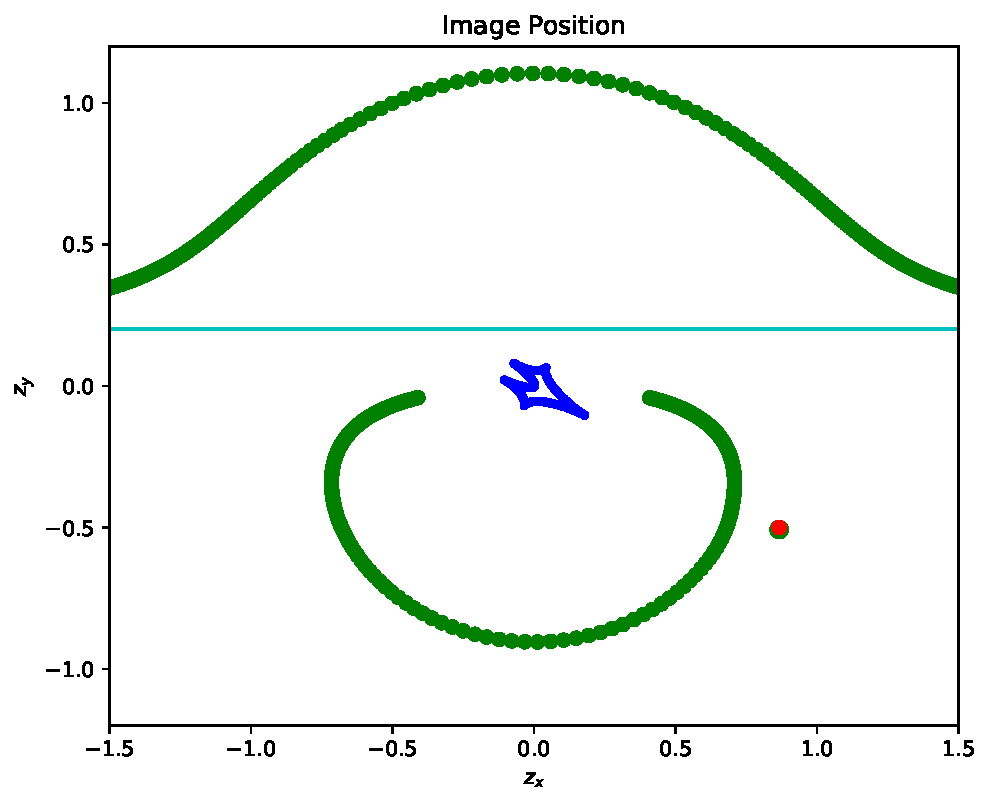
\includegraphics[width=7 cm]{Image_and_Caustic_Curves_x_sqrt3_2_-0_5j.pdf}
  \end{minipage}\hfill
\end{subfigure}%
\begin{subfigure}{.5\textwidth}
  \begin{minipage}{0.1\textwidth}
    \caption{} \label{fig:Magnification_sqrt3_2_-0_5j}
  \end{minipage}\hfill
\begin{minipage}[c]{0.85\textwidth}
    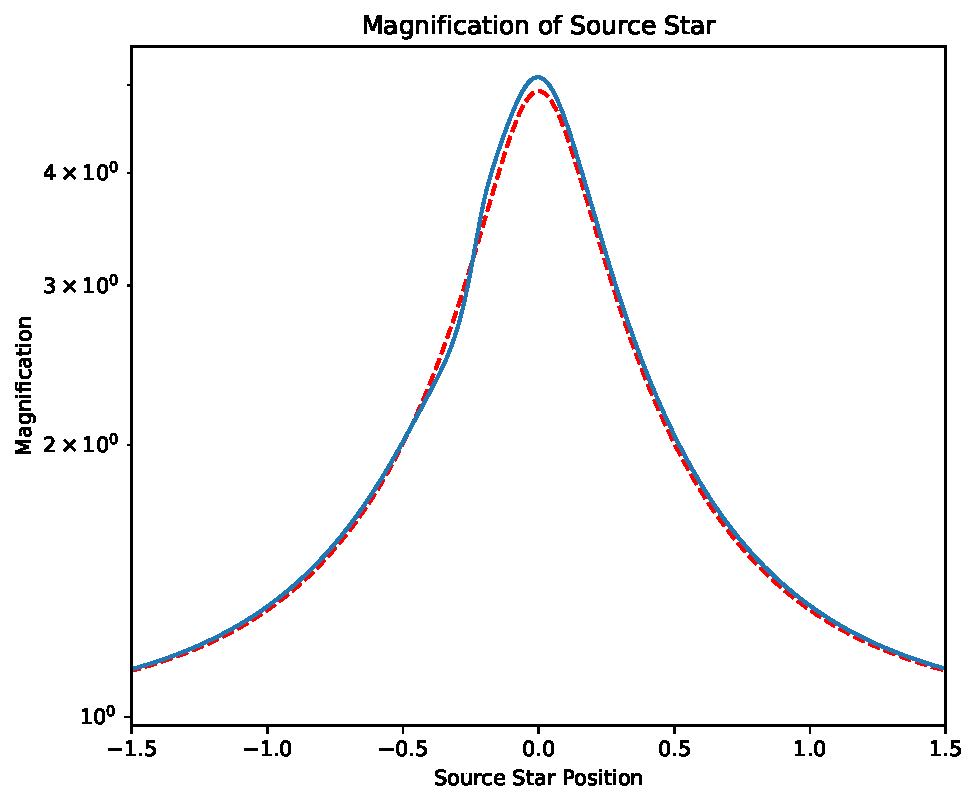
\includegraphics[width=7 cm]{Magnification_x_sqrt3_2_-0_5j.pdf}
  \end{minipage}\hfill
\end{subfigure} %
\captionsetup{justification=centering}
\caption{\label{fig:Image_and_Magnification} Caustic curves were plotted in blue, the green curves denote the image of the source star whose trajectory is shown in cyan. The lens star was positioned at the origin and the planet is denoted by the red circle. The leftmost figures show the images of the source star as it transitions behind the lens star at a $y$ position of 0.2 $\theta_E$. The planets are positioned at ${(x,y) = (1.2,0.5)~\theta_E}$, ${(x,y) = (1.2,-0.5)~\theta_E}$, and ${(x,y) = (\sqrt{3}/2,-0.5)~\theta_E}$, for Figs.~\ref{fig:Image_1_2_0_5j}, \ref{fig:Image_1_2_n0_5j}, and \ref{fig:Image_sqrt3_2_n0_5j} respectively. The rightmost figures show the magnification of the source star by the lens star and planet, as shown in blue. For each of the three figures the magnification is perturbed from the single lens case shown in red.}
\end{figure}



\end{document}